\section{Modeling and Controlling ATSs - The MPC for ATS and the RCS} 

% ==================///==================///==================///
\begin{frame}{How can the CATSM shortcomings be solved?}
	Three combined approaches
	\vspace{0.5cm}
	\begin{itemize}
		\item Novel linear discrete-time model
		\item Definition of an ad-hoc model predictive control (MPC) 
		\item Adaptive road network optimization using graph transformation systems (GTS)
	\end{itemize}
\end{frame}

% ==================///==================///==================///
\begin{frame}{Novel Model for ATSs}
	Key idea $\rightarrow$ Define AVs speed in function of the number of AVs currently on the street
	\begin{columns}
		\begin{column}{0.4\textwidth}
			\begin{equation*}
				\resizebox{1.3\textwidth}{!}{$
				\begin{aligned}	
					s_{ij}(V_{ij}) &= \begin{cases}
						l_{ij} \quad\quad &\text{if } V_{ij}\in[0,V_{ij}^{th})\\ 
						l_{ij} - b\cdot(V_{ij}^{th}- V_{ij}) \quad\quad &\text{if }V_{ij}\in[V_{ij}^{th}, V_{ij}^{max})\\ 
						0\quad\quad &\text{if }V_{ij} \ge V_{ij}^{max}\\ 
					\end{cases}\\
					\text{with } b  &=  \dfrac{l_{ij}-\epsilon }{ V_{ij}^{th} -  V_{ij}^{max}} \text{ and } \epsilon \in (0,1)
				\end{aligned}
				$}
			\end{equation*}
			$\rightarrow$ Implicitely, a better congestion model
		\end{column}
		\begin{column}{0.4\textwidth}
			\begin{figure}[t]
				\centering
				\resizebox{1.1\textwidth}{!}{
				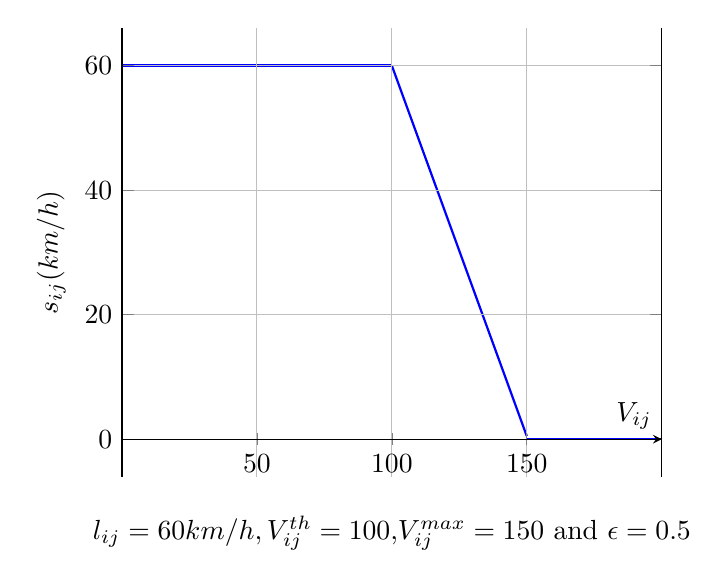
\begin{tikzpicture}
					\begin{axis}[
						xlabel={$V_{ij}$},
						ylabel={$s_{ij} (km/h)$},
						domain=0:250, % adjust the domain based on your preference
						samples=40,
						grid=both,
						axis x line=middle,
						%ymin=-1, % Set the minimum y-axis value
						%ymax=1.4, % Set the maximum y-axis value
						axis on top,
						legend pos=north east,
						title style={at={(0.5,-0.1)},anchor=north,yshift=-0.5},
						title={$l_{ij} = 60 km/h,V_{ij}^{th} = 100$,$V_{ij}^{max} = 150$ and $\epsilon = 0.5$},
						]
						% Piecewise function
						\addplot[blue, thick, domain=0:100] {60};
						\addplot[blue, thick, domain=100:150] {60 - 1.19*(x-100)};
						\addplot[blue, thick, domain=150:200] {0};
						%\addlegendentry{B}
					\end{axis}
				\end{tikzpicture}
			}
			\end{figure}
		\end{column}
	\end{columns}
\end{frame}

% ==================///==================///==================///
\begin{frame}{Novel Model for ATSs}
	As a result, new model linear time-discrete model can be defined, which tracks
	\begin{itemize}
		\item AVs' position using the speed 
		\item Stationed AVs
		\item Served and Unserved requests using travelling vehicles
	\end{itemize}
	\vspace{0.3cm}
	$\rightarrow$ System can be controlled by determining number of vehicles circulating
\end{frame}


% ==================///==================///==================///
\begin{frame}{Model Predictive Control for ATSs}
	Let $\mathcal{X}$ and $\mathcal{U}$ being the set of feasible states and inputs, respectively, solve
	\begin{equation}
		\begin{aligned}
			\underset{\substack{u(t), \dots, u(t+N)}}{\text{\textbf{min}}} \quad & J_f(x(N))+\sum_{t=0}^{N-1}I(x(t)) \\
			\text{\textbf{s.t.}} \quad & x(t+1) = Ax(t) + Bu(t)  \\
			& x(t) \in \mathcal{X}, \ u(t)\in \mathcal{U} \\
			%& k = t, \dots, t+N\\
			&x(N) \in \mathcal{X}_f\\
		\end{aligned}
	\end{equation}
	%where $\mathcal{X}_f$ is the set of terminal states, $J_f(x(N))$ is the terminal cost function and $I(x(t))$ is the stage cost. 
	\vspace{0.7cm}
	$\rightarrow$ Lyapunov stability can be proven
\end{frame}
% ==================///==================///==================///
\begin{frame}{Model Predictive Control for ATSs}
	New control strategy possible which
	\vspace{0.1cm}
	\hspace{9.5 cm}\tikzmark{right}
	\begin{itemize}
		\item Reduces number of outstanding requests \tikzmark{a}
		\item Minimizes unnecessary rebalancing vehicles \tikzmark{b}
		\vspace{0.2cm}
		\item Avoids transportation after requests are served \tikzmark{c}
		\item Avoids rebalancing after requests are served \tikzmark{d}
	\end{itemize}
	
	\begin{tikzpicture}[overlay, remember picture]
		\node[anchor=base] (1) at (pic cs:a) {\vphantom{h}}; % push the mark to the top of the line (ie including ascenders)
		\node[anchor=base] (2) at (pic cs:b) {\vphantom{g}}; % push the mark to the bottom of the line (ie including descenders)
		\node[anchor=base] (3) at (pic cs:c) {\vphantom{h}}; % push the mark to the top of the line (ie including ascenders)
		\node[anchor=base] (4) at (pic cs:d) {\vphantom{g}}; % push the mark to the bottom of the line (ie including descenders)
		\draw [decoration={brace,amplitude=0.5em},decorate,ultra thick,black]
		(1.north -| {pic cs:right}) -- (2.south -| {pic cs:right}) node[midway, right=1em] {Combined give $I(x(t))$};
		\draw [decoration={brace,amplitude=0.5em},decorate,ultra thick,black]
		(3.north -| {pic cs:right}) -- (4.south -| {pic cs:right}) node[midway, right=1em] {Combined give $J_f(x(N))$};
	\end{tikzpicture}
\end{frame}

% ==================///==================///==================///
\begin{frame}{Reduced Connectivity Schema}
	So far
	\begin{itemize}
		\item More sophisticated congestion model \checkmark
		\item Gained insights into the future of the system \checkmark
	\end{itemize}
	$\rightarrow$ What about scalability?\\
	\vspace{0.5cm}
	Solution: Reduced Connectivity Schema (RCS). \\
	\vspace{0.1cm}
	In a nutshell, create a condensed version of $G$  using a sequence of transformation rules $\mathcal{T}$.
\end{frame}
% ==================///==================///==================///
\begin{frame}{Constructing an RCS}
	%Rules are highly application-dependent, therefore let's assume the NYC road network used prior. \\
	%\vspace{0.2cm}
	%Applied rules starting from only the important nodes
	Rules that have been applie
	\begin{enumerate}
		\item Restoration of important nodes' immidiate connections 
		\item Restoration of simpe nodes' immidiate connections (iteratively)\label{rule2}
		\item Straight Line Node elimination
		\item Dead-End Removal
	\end{enumerate}
	\vspace{0.2cm}
	$\rightarrow$ Depending on rule \ref{rule2}, the RCS may comprise as little as 18\% of the original road network's size.
	
\end{frame}

% ==================///==================///==================///
%\begin{frame}{MPC for ATSs}
%	Let $V_{ij}(t) \in \{ x \in \mathbb{N}_0 : x \leq |\mathcal{A}|\}$ being the total number of vehicles currently circulating on the street $\langle i,j\rangle$, this can be easily computed by adding the number of carries to the rebalancing AVs, i.e. \\
%	\begin{equation*}
%		V_{ij}(t) = \sum_{a \in \mathcal{A}} v^{a}_{ij}(t) +w^{a}_{ij}(t)
%	\end{equation*}
%	$\rightarrow$ Control  $v^{a}_{ij}(t)$ and $w^{a}_{ij}(t)$
%\end{frame}






% ==================///==================///==================///
\begin{frame}{Evaluation}
	\hspace{0.5cm} Good basis that can be further expanded
	\vspace{0.5cm}
	\begin{columns}
		\begin{column}{0.35\textwidth}
			
			\begin{itemize}
				\item[+] More descriptive model
				\item[+] Optimal control law guaranteed
				\item[+] Can ``predict'' the future
			\end{itemize}
		\end{column}
		%%
		\vline
		\hspace{0.8cm}
		\begin{column}{0.4\textwidth}
			\begin{itemize}
				\item[-] The model is not tracking non-driving entities (e.g., pedestrians, cyclists)
				\item[-] Special vehicles not considered (e.g., ambulances)
				\item[-] Must be expanded further
			\end{itemize}
		\end{column}
	\end{columns}
\end{frame}



